\documentclass[a4paper, 11pt, amsmath, graphicx]{article}\usepackage[]{graphicx}\usepackage[]{color}
%% maxwidth is the original width if it is less than linewidth
%% otherwise use linewidth (to make sure the graphics do not exceed the margin)
\makeatletter
\def\maxwidth{ %
  \ifdim\Gin@nat@width>\linewidth
    \linewidth
  \else
    \Gin@nat@width
  \fi
}
\makeatother

\definecolor{fgcolor}{rgb}{0.345, 0.345, 0.345}
\newcommand{\hlnum}[1]{\textcolor[rgb]{0.686,0.059,0.569}{#1}}%
\newcommand{\hlstr}[1]{\textcolor[rgb]{0.192,0.494,0.8}{#1}}%
\newcommand{\hlcom}[1]{\textcolor[rgb]{0.678,0.584,0.686}{\textit{#1}}}%
\newcommand{\hlopt}[1]{\textcolor[rgb]{0,0,0}{#1}}%
\newcommand{\hlstd}[1]{\textcolor[rgb]{0.345,0.345,0.345}{#1}}%
\newcommand{\hlkwa}[1]{\textcolor[rgb]{0.161,0.373,0.58}{\textbf{#1}}}%
\newcommand{\hlkwb}[1]{\textcolor[rgb]{0.69,0.353,0.396}{#1}}%
\newcommand{\hlkwc}[1]{\textcolor[rgb]{0.333,0.667,0.333}{#1}}%
\newcommand{\hlkwd}[1]{\textcolor[rgb]{0.737,0.353,0.396}{\textbf{#1}}}%

\usepackage{framed}
\makeatletter
\newenvironment{kframe}{%
 \def\at@end@of@kframe{}%
 \ifinner\ifhmode%
  \def\at@end@of@kframe{\end{minipage}}%
  \begin{minipage}{\columnwidth}%
 \fi\fi%
 \def\FrameCommand##1{\hskip\@totalleftmargin \hskip-\fboxsep
 \colorbox{shadecolor}{##1}\hskip-\fboxsep
     % There is no \\@totalrightmargin, so:
     \hskip-\linewidth \hskip-\@totalleftmargin \hskip\columnwidth}%
 \MakeFramed {\advance\hsize-\width
   \@totalleftmargin\z@ \linewidth\hsize
   \@setminipage}}%
 {\par\unskip\endMakeFramed%
 \at@end@of@kframe}
\makeatother

\definecolor{shadecolor}{rgb}{.97, .97, .97}
\definecolor{messagecolor}{rgb}{0, 0, 0}
\definecolor{warningcolor}{rgb}{1, 0, 1}
\definecolor{errorcolor}{rgb}{1, 0, 0}
\newenvironment{knitrout}{}{} % an empty environment to be redefined in TeX

\usepackage{alltt}
% R vignette preable

\usepackage{amsmath}
\usepackage{mathtools}
\usepackage{amsfonts}
\usepackage{amssymb}
\usepackage{hyperref}

\usepackage{geometry}
 \geometry{
 a4paper,
 total={170mm,257mm},
 left=20mm,
 top=20mm,
 }
 
\usepackage{fancyhdr}
\pagestyle{fancy}
\renewcommand{\headrulewidth}{0pt}
\renewcommand{\footrulewidth}{0pt}
\setlength\headheight{80.0pt}
\addtolength{\textheight}{-80.0pt}
\lhead{
\includegraphics[width=0.34\textwidth]{UoLLogoMono.pdf}}

\def\bmu{{\mbox{\boldmath $\mu$}}}
\def\bt{{\mbox{\boldmath $\theta$}}}
\def\bs{{\mbox{\boldmath $\sigma$}}}
\IfFileExists{upquote.sty}{\usepackage{upquote}}{}
\begin{document}
\title{4. Real data}
\author{Simon Vaughan \thanks{Email: sav2@le.ac.uk}}
\maketitle

In this section we discuss an example of a real astronomical dataset.

%%%%%%%%%%%%%%%%%%%%%%%%%%%%%%%%%%%%%%%%%%%%%%%%%%%%%%%%%%%%%%%%%%%%%%5
\vspace{0.4cm}
\textbf{The observations}
\\

During 2016 the \emph{Swift} satellite made repeated observations of the active galaxy NGC 6814 as part of a Leicester-led project. We obtained data from $n = 43$ short observations, which provided fluxes (a measure of brightness) in X-ray and ultraviolet (UV) wavebands. Here we will look at both of these.

The data file {\tt 2016\_uvw1\_rate.txt} is an ASCII (plain text) file containing 4 columns of numbers, and a first row with the column names (a \emph{header} row). The columns give
\begin{enumerate}
\item {\tt t}: the observation time in Modified Julian Day (MJD)
\item {\tt dt}: the length of the observation (in days)
\item {\tt y}: the flux (brightness) in counts second$^{-1}$ units
\item {\tt dy}: the error on the flux in counts second$^{-1}$ units
\end{enumerate}

We can use R to load the data file and make a simple plot.

\begin{knitrout}
\definecolor{shadecolor}{rgb}{0.969, 0.969, 0.969}\color{fgcolor}\begin{kframe}
\begin{alltt}
\hlcom{# set the working directory}
\hlkwd{setwd}\hlstd{(}\hlstr{"C:/Users/sav2/Documents/R/gin/vignettes"}\hlstd{)}

\hlcom{# load the file into the 'dat' object}
\hlstd{dat} \hlkwb{<-} \hlkwd{read.table}\hlstd{(}\hlstr{"2016_uvw1_rate.txt"}\hlstd{,} \hlkwc{header} \hlstd{=} \hlnum{TRUE}\hlstd{)}

\hlcom{# subtract the start time}
\hlstd{dat}\hlopt{$}\hlstd{t} \hlkwb{<-} \hlstd{dat}\hlopt{$}\hlstd{t} \hlopt{-} \hlkwd{min}\hlstd{(dat}\hlopt{$}\hlstd{t)}

\hlcom{# plot the data}
\hlkwd{plot}\hlstd{(dat}\hlopt{$}\hlstd{t, dat}\hlopt{$}\hlstd{y,} \hlkwc{bty} \hlstd{=} \hlstr{"n"}\hlstd{,} \hlkwc{xlab} \hlstd{=} \hlstr{"time (days)"}\hlstd{,} \hlkwc{ylab} \hlstd{=} \hlstr{"UV flux"}\hlstd{)}

\hlcom{# add the error bars to the plot}
\hlkwd{segments}\hlstd{(dat}\hlopt{$}\hlstd{t, dat}\hlopt{$}\hlstd{y} \hlopt{-} \hlstd{dat}\hlopt{$}\hlstd{dy, dat}\hlopt{$}\hlstd{t, dat}\hlopt{$}\hlstd{y} \hlopt{+} \hlstd{dat}\hlopt{$}\hlstd{dy)}
\end{alltt}
\end{kframe}

{\centering 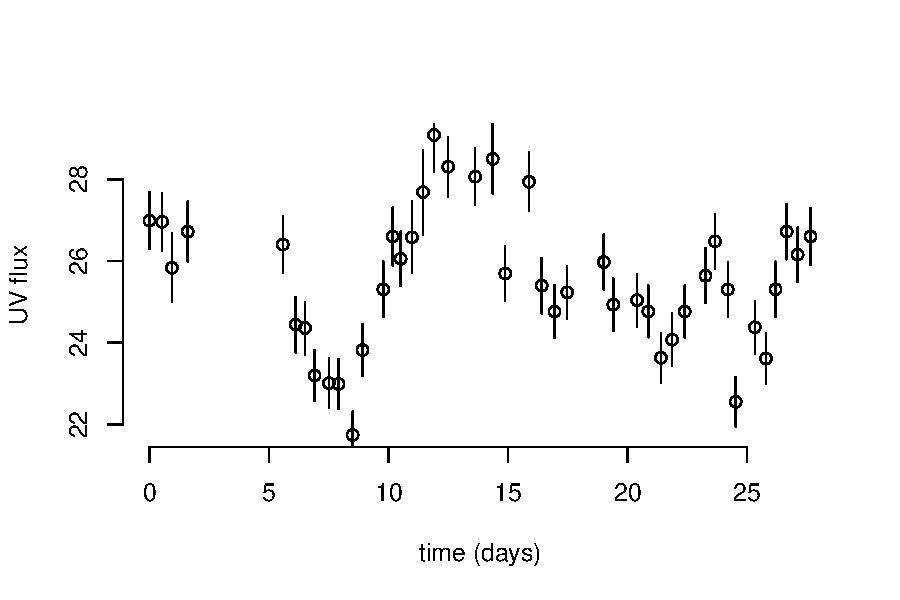
\includegraphics[width=\maxwidth]{figure/unnamed-chunk-1-1} 

}



\end{knitrout}

The times are not evenly spaced, and the errors {\tt dy} are different for each observations. We should be able to account for both of these properties of the data quite naturally using a Gaussian Process model.

And we can do the same with the X-ray data from the file {\tt 2016\_xrt\_rate.txt} which is in exactly the same format.

\begin{knitrout}
\definecolor{shadecolor}{rgb}{0.969, 0.969, 0.969}\color{fgcolor}\begin{kframe}
\begin{alltt}
\hlcom{# load the file into the 'dat' object}
\hlstd{dat} \hlkwb{<-} \hlkwd{read.table}\hlstd{(}\hlstr{"2016_xrt_rate.txt"}\hlstd{,} \hlkwc{header} \hlstd{=} \hlnum{TRUE}\hlstd{)}

\hlcom{# subtract the start time}
\hlstd{dat}\hlopt{$}\hlstd{t} \hlkwb{<-} \hlstd{dat}\hlopt{$}\hlstd{t} \hlopt{-} \hlkwd{min}\hlstd{(dat}\hlopt{$}\hlstd{t)}

\hlcom{# plot the data}
\hlkwd{plot}\hlstd{(dat}\hlopt{$}\hlstd{t, dat}\hlopt{$}\hlstd{y,} \hlkwc{bty} \hlstd{=} \hlstr{"n"}\hlstd{,} \hlkwc{xlab} \hlstd{=} \hlstr{"time (days)"}\hlstd{,} \hlkwc{ylab} \hlstd{=} \hlstr{"X-ray flux"}\hlstd{)}

\hlcom{# add the error bars to the plot}
\hlkwd{segments}\hlstd{(dat}\hlopt{$}\hlstd{t, dat}\hlopt{$}\hlstd{y} \hlopt{-} \hlstd{dat}\hlopt{$}\hlstd{dy, dat}\hlopt{$}\hlstd{t, dat}\hlopt{$}\hlstd{y} \hlopt{+} \hlstd{dat}\hlopt{$}\hlstd{dy)}
\end{alltt}
\end{kframe}

{\centering 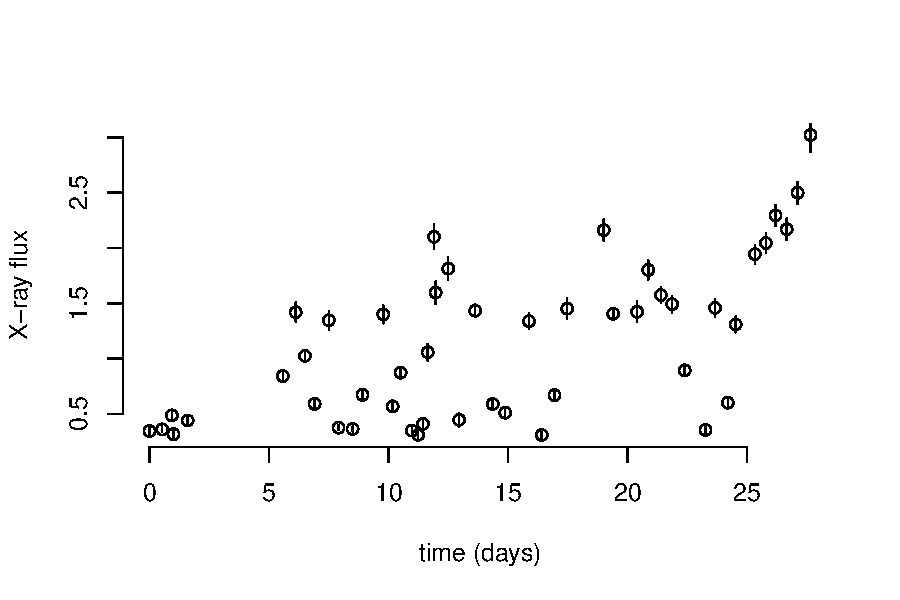
\includegraphics[width=\maxwidth]{figure/unnamed-chunk-2-1} 

}



\end{knitrout}

Notice how much more variable the X-rays are, so we make a logarithmic transformation to the axis and re-plot.


\begin{knitrout}
\definecolor{shadecolor}{rgb}{0.969, 0.969, 0.969}\color{fgcolor}\begin{kframe}
\begin{alltt}
\hlcom{# plot the data}
\hlkwd{plot}\hlstd{(dat}\hlopt{$}\hlstd{t, dat}\hlopt{$}\hlstd{y,} \hlkwc{bty} \hlstd{=} \hlstr{"n"}\hlstd{,} \hlkwc{xlab} \hlstd{=} \hlstr{"time (days)"}\hlstd{,} \hlkwc{ylab} \hlstd{=} \hlstr{"X-ray flux"}\hlstd{,} \hlkwc{log} \hlstd{=} \hlstr{"y"}\hlstd{)}

\hlcom{# add the error bars to the plot}
\hlkwd{segments}\hlstd{(dat}\hlopt{$}\hlstd{t, dat}\hlopt{$}\hlstd{y} \hlopt{-} \hlstd{dat}\hlopt{$}\hlstd{dy, dat}\hlopt{$}\hlstd{t, dat}\hlopt{$}\hlstd{y} \hlopt{+} \hlstd{dat}\hlopt{$}\hlstd{dy)}
\end{alltt}
\end{kframe}

{\centering 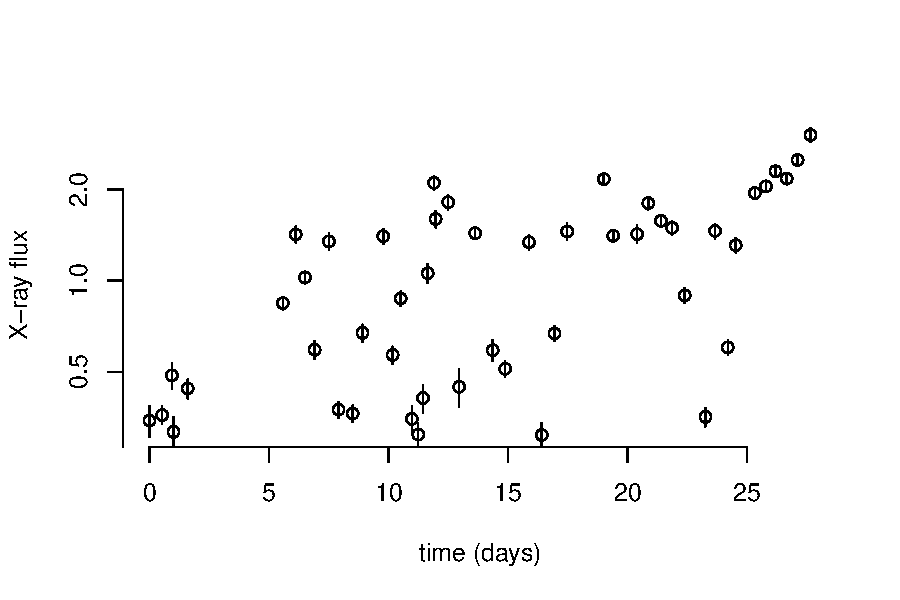
\includegraphics[width=\maxwidth]{figure/unnamed-chunk-3-1} 

}



\end{knitrout}

Clearly the processes that generates the X-ray and UV variations are quite different; the X-ray variations are much stronger (larger amplitude) and more rapid (less smooth). We would like to be able to infer the properties of the random processes at work here. If we assume these are stationary GPs then the only important characteristic is the auto-covariance function $ACV(\tau)$. 

If we think the X-rays are produced by a lognormal process (i.e. $\ln \mathbf{y} \sim N(\mu, \Sigma)$), we can treat this by modelling the logarithm of the fluxes (i.e. we apply a simple log transformation to the data, and the corresponding transformation to the errors, prior to fitting with a GP model).

%%%%%%%%%%%%%%%%%%%%%%%%%%%%%%%%%%%%%%%%%%%%%%%%%%%%%%%%%%%%%%%%%%%%%%5
\vspace{0.4cm}
\textbf{The errors}
\\

A further point is that sometimes we cannot trust the error bars. In the case of the \emph{Swift} data here, the errors are usually quite reliable indicators of the reproduceability of the data. But data taken from other telescopes can be less reliable. To account for this we can allow an additional parameter $\nu$ that is a multiplicative factor applied to the errors. I.e. the covariance matrix of the measurement `noise' is:

\begin{align}
 N & = \nu \bs^2 I_n, \nonumber \\
 N_{ij} & = \nu \sigma_i^2 \delta_{ij}.
\end{align}

And we should find $\nu \approx 1$ when the error bars are reliable. The covariance matrix for the GP model is then 

\begin{equation}
  \Sigma = K + N.
\end{equation}

\end{document}
